\documentclass{beamer}

\usepackage{changepage}
\usepackage{subcaption}
%\usepackage[demo]{graphicx}
%\usepackage{floatrow}
\usepackage{sidecap}

\setbeamertemplate{caption}{\insertcaption}

\title{Improved scaling of the disk space taken by the Bitcoin blockchain}
\date{}%juin 2021}
\author{Benjamin Loison}

\addtobeamertemplate{navigation symbols}{}
{
    \usebeamerfont{footline}
    \usebeamercolor[fg]{footline}
    \hspace{1em}
    \insertframenumber/\inserttotalframenumber
}

\setbeamercolor{footline}{fg=blue}
\setbeamerfont{footline}{series=\bfseries}

\begin{document}

\frame{\titlepage}

%\begin{frame}
%\frametitle{Table of Contents}
%\tableofcontents
%\end{frame}

\begin{frame}

\frametitle{Introduction to blockchains}

\begin{figure}
\centering
\begin{subfigure}{.5\textwidth}
  \centering
  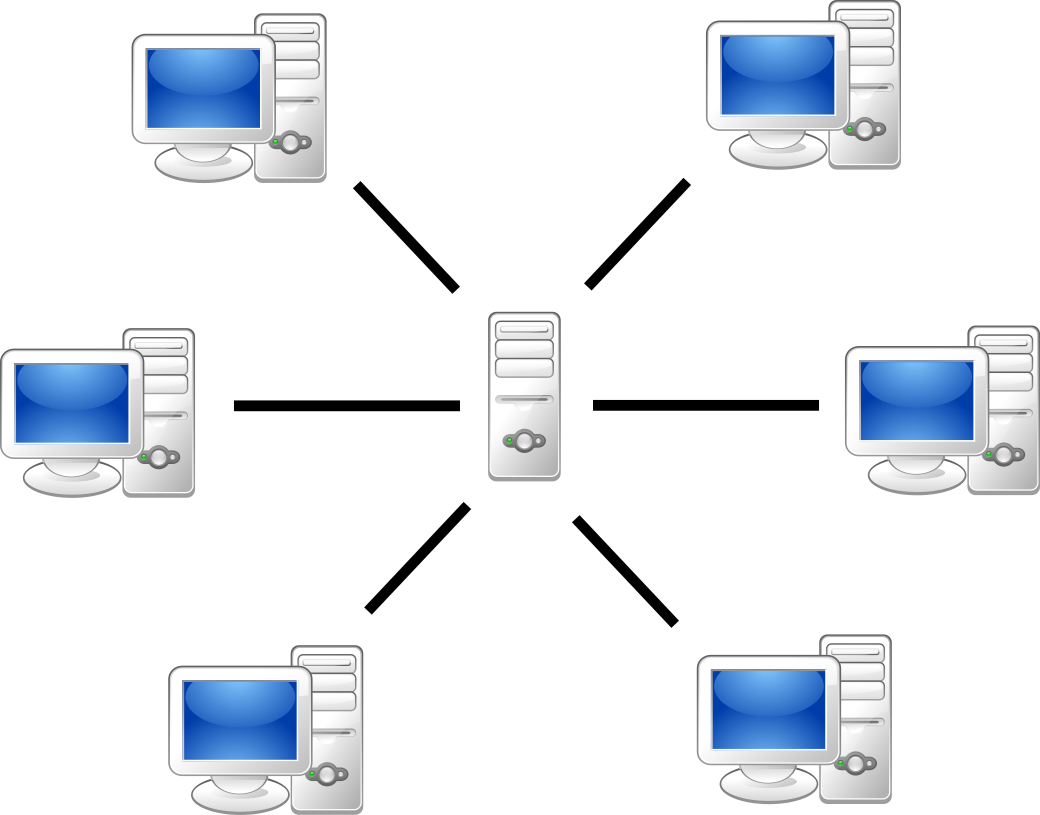
\includegraphics[width=.8\linewidth]{illustrationsSoutenance/clientServer.png}
  \caption{Master-slave network}
  \label{fig:sub1}
\end{subfigure}% if remove this comment it doesn't work anymore
\begin{subfigure}{.5\textwidth}
  \centering
  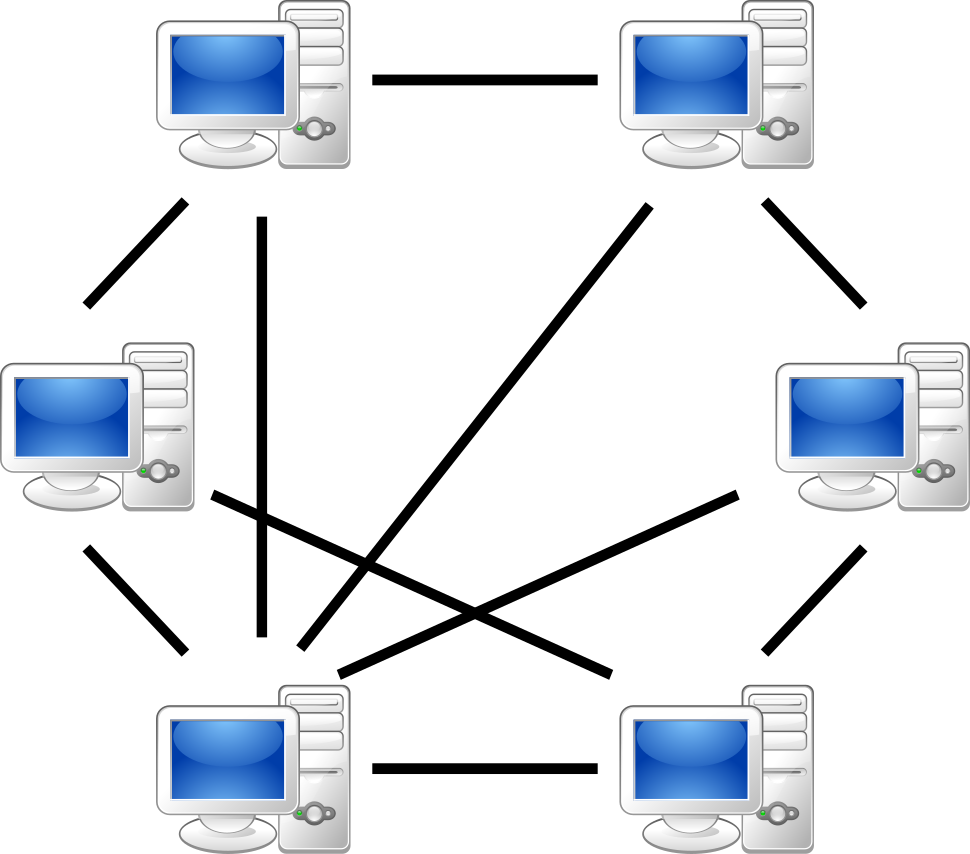
\includegraphics[width=.8\linewidth]{illustrationsSoutenance/P2P.png}
  \caption{Peer-to-peer network}
  \label{fig:sub2}
\end{subfigure}
\end{figure}
\end{frame}

%\newpage

\begin{frame}

\frametitle{The scalability problem}

\begin{figure}[H]
		%\caption{Taille de la blockchain de Bitcoin en fonction du temps}
		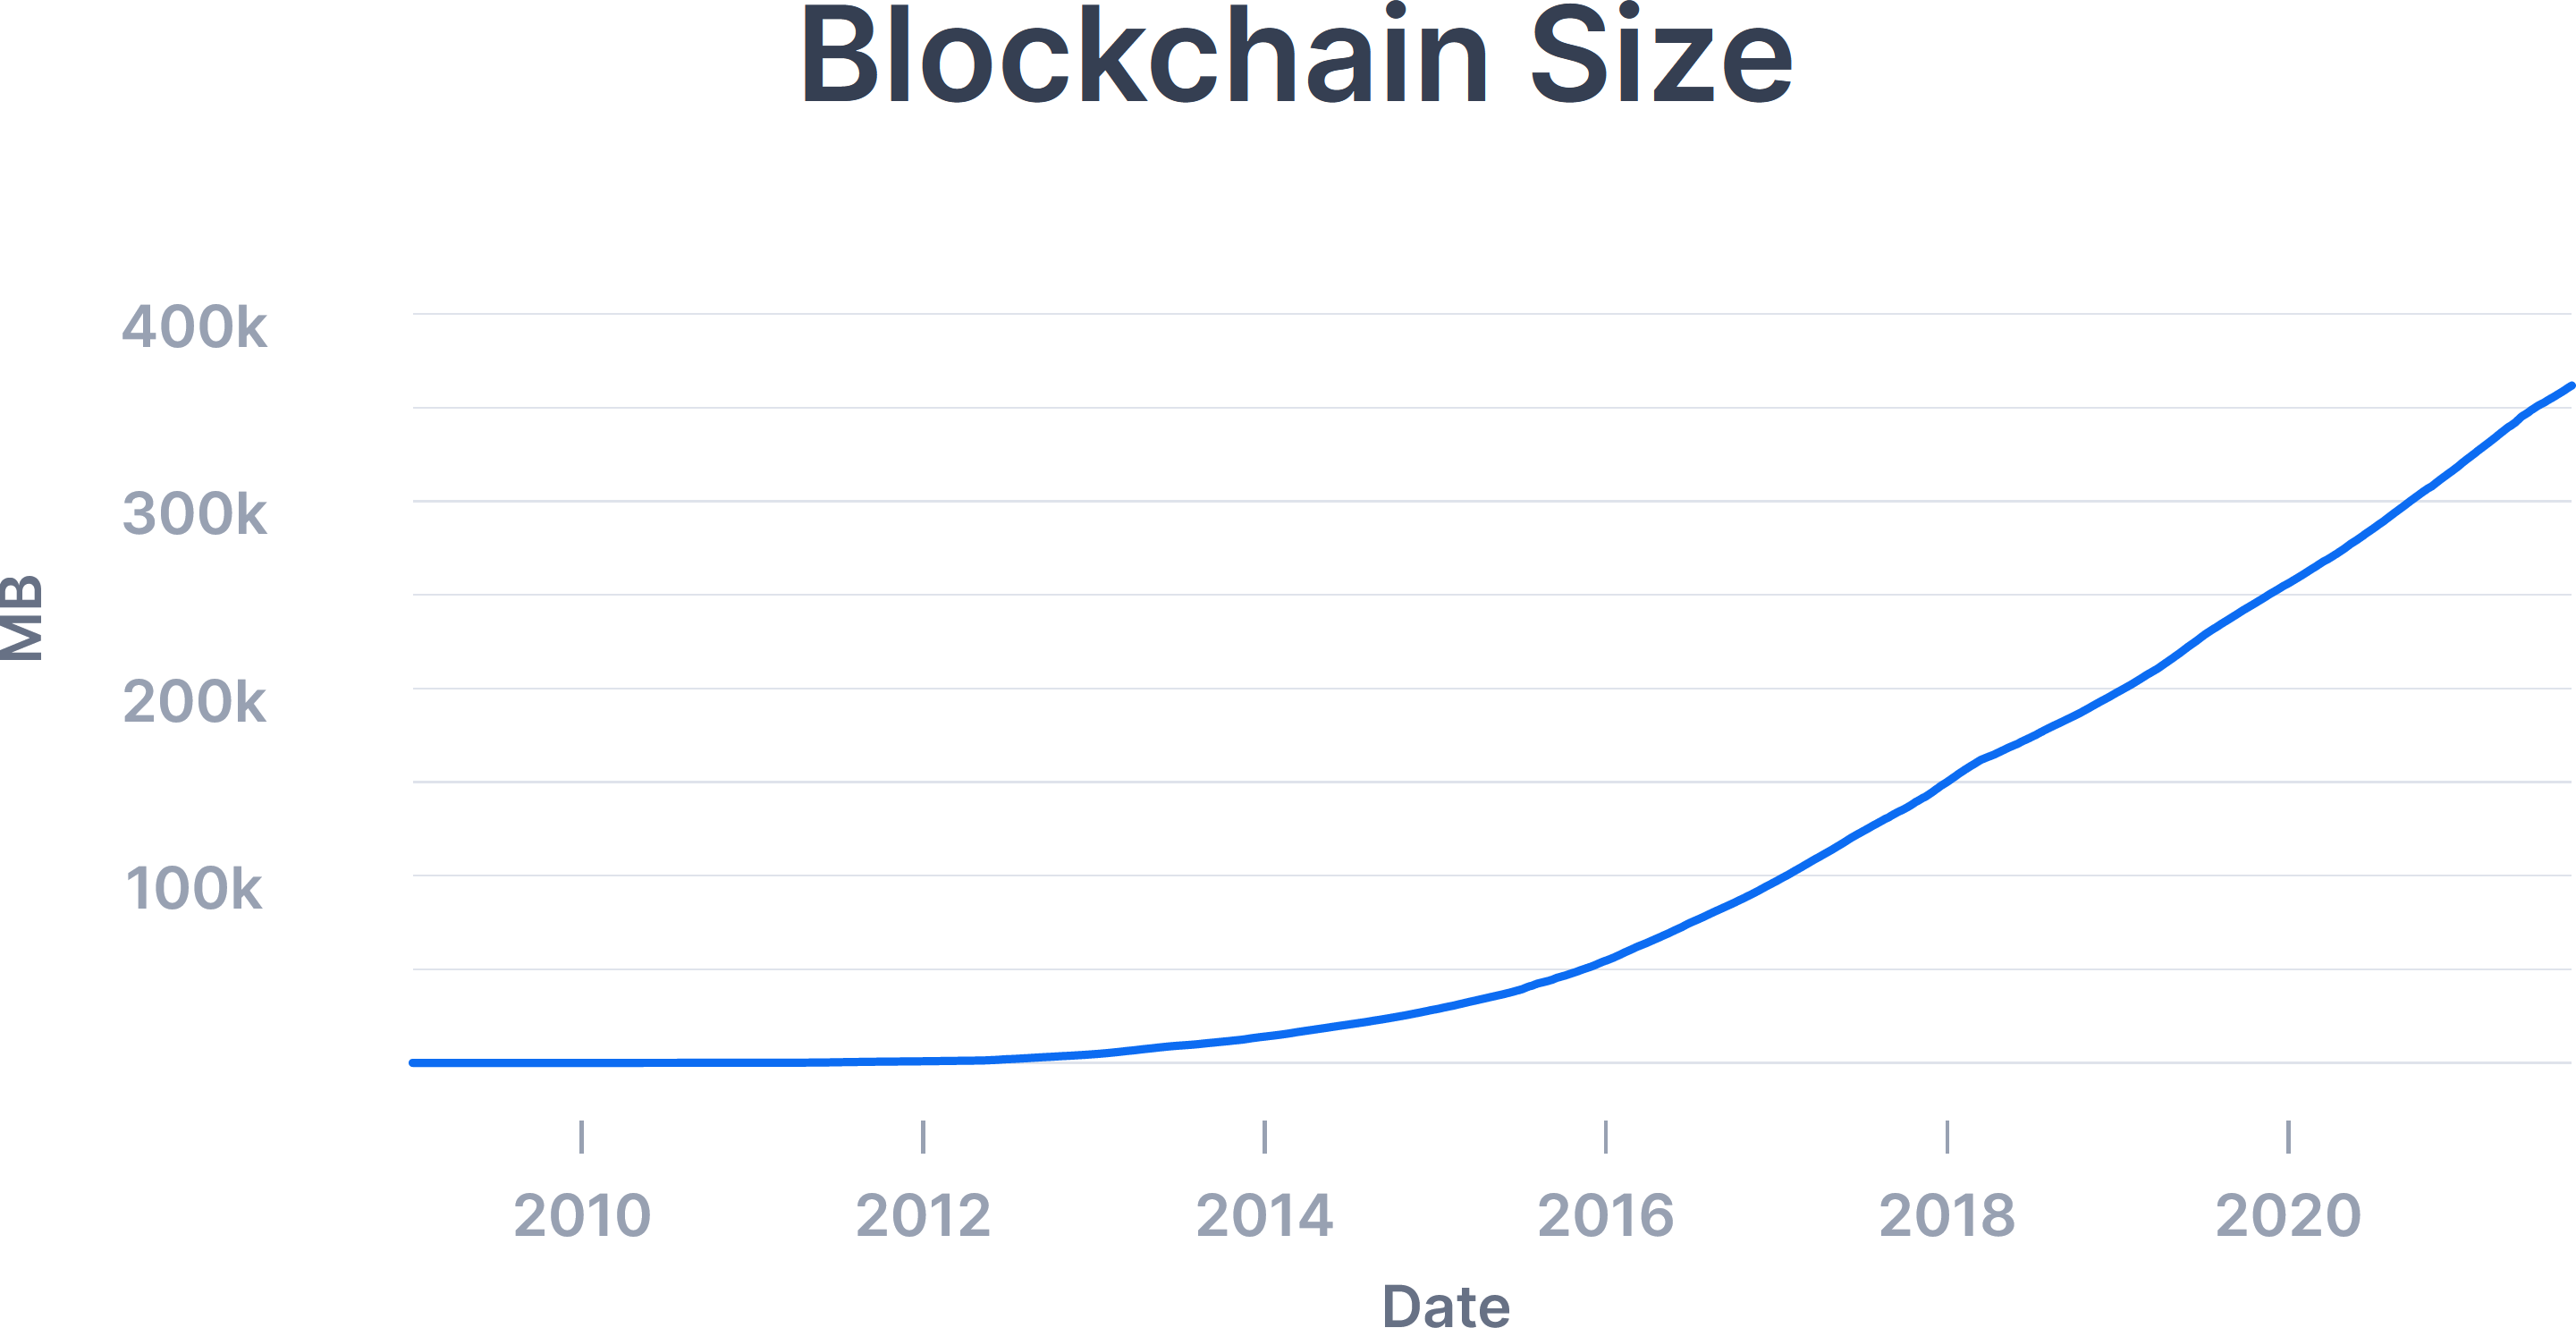
\includegraphics[width=\linewidth]{illustrationsSoutenance/blockchainSizeSourceless.png}
	\end{figure}

\end{frame}

\begin{frame}

\frametitle{The idea of the internship}

\begin{itemize}
	\item Mining in Logarithmic Space 2021 Aggelos Kiayias, Nikos Leonardos and Dionysis Zindros
\end{itemize}

\begin{figure}[H]
		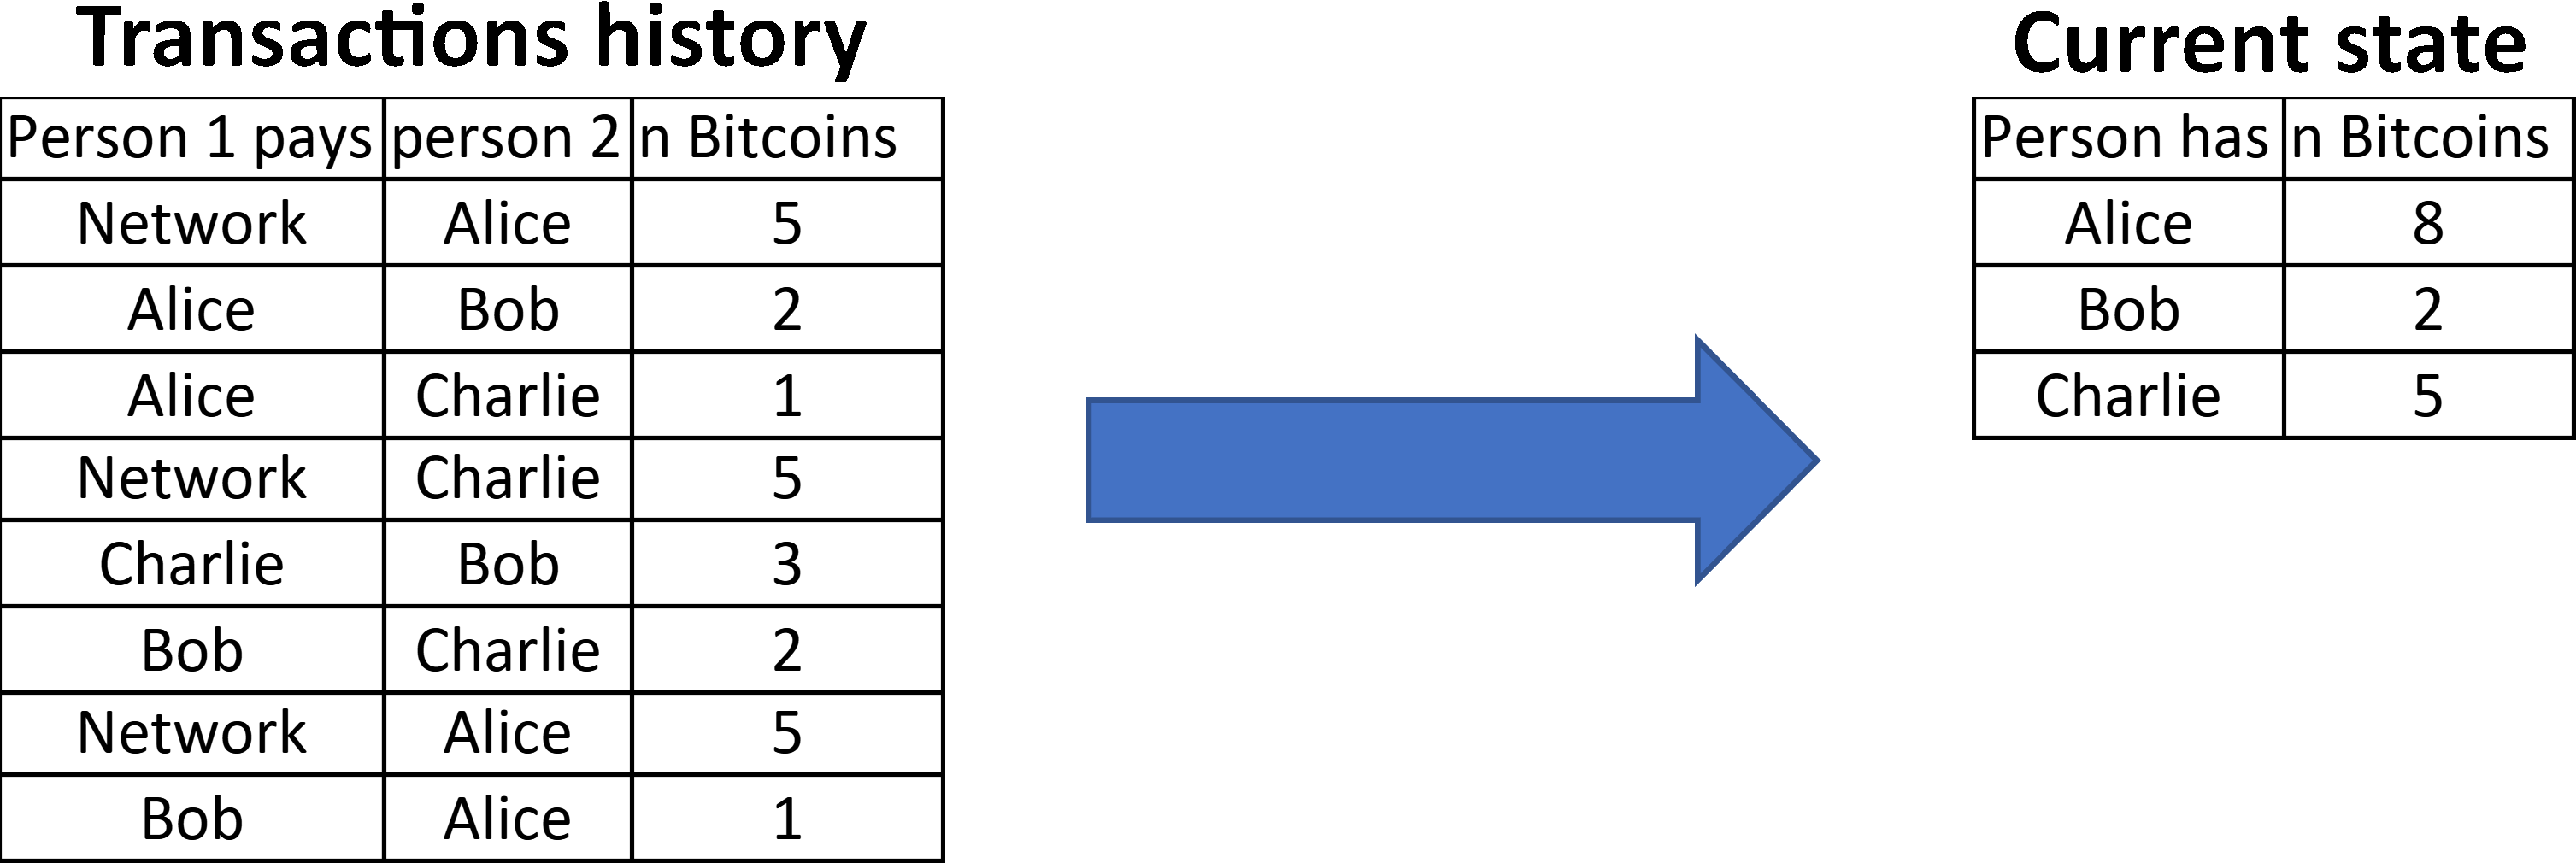
\includegraphics[width=\linewidth]{illustrationsSoutenance/ideaTitleEN.png}
	\end{figure}

\end{frame}


\begin{frame}

\frametitle{How Bitcoin works}

\begin{figure}[H]
		\includegraphics[width=\linewidth]{illustrationsSoutenance/blockchainEN.png}
	\end{figure}

\end{frame}


\begin{frame}

\frametitle{Mining blocks}

Data:\\
\vspace{0.5cm}

Block 0 n\\
Alice earns 5 BTC\\
Alice pays Bob 2 BTC\\
Alice pays Charlie 1 BTC\\

\vspace{0.5cm}
\begin{tabular}{| c | c |}
	\hline
   n     & SHA-256² hash\\ \hline
   0     & 6c7c2450bd52e950a3db47d8dc91cbdb04a792561759\dots \\ \hline
   1     & 6442a403b0cd2bac7b3af363a342769d1955f9851d65\dots \\ \hline
   \dots & \dots \\ \hline
   86    & 00e9d707e8f386a73d2455cfa9c06d618285f03e434a\dots\\
	\hline
 \end{tabular}

\end{frame}


\begin{frame}

\frametitle{The fork problem}

\begin{figure}[H]
		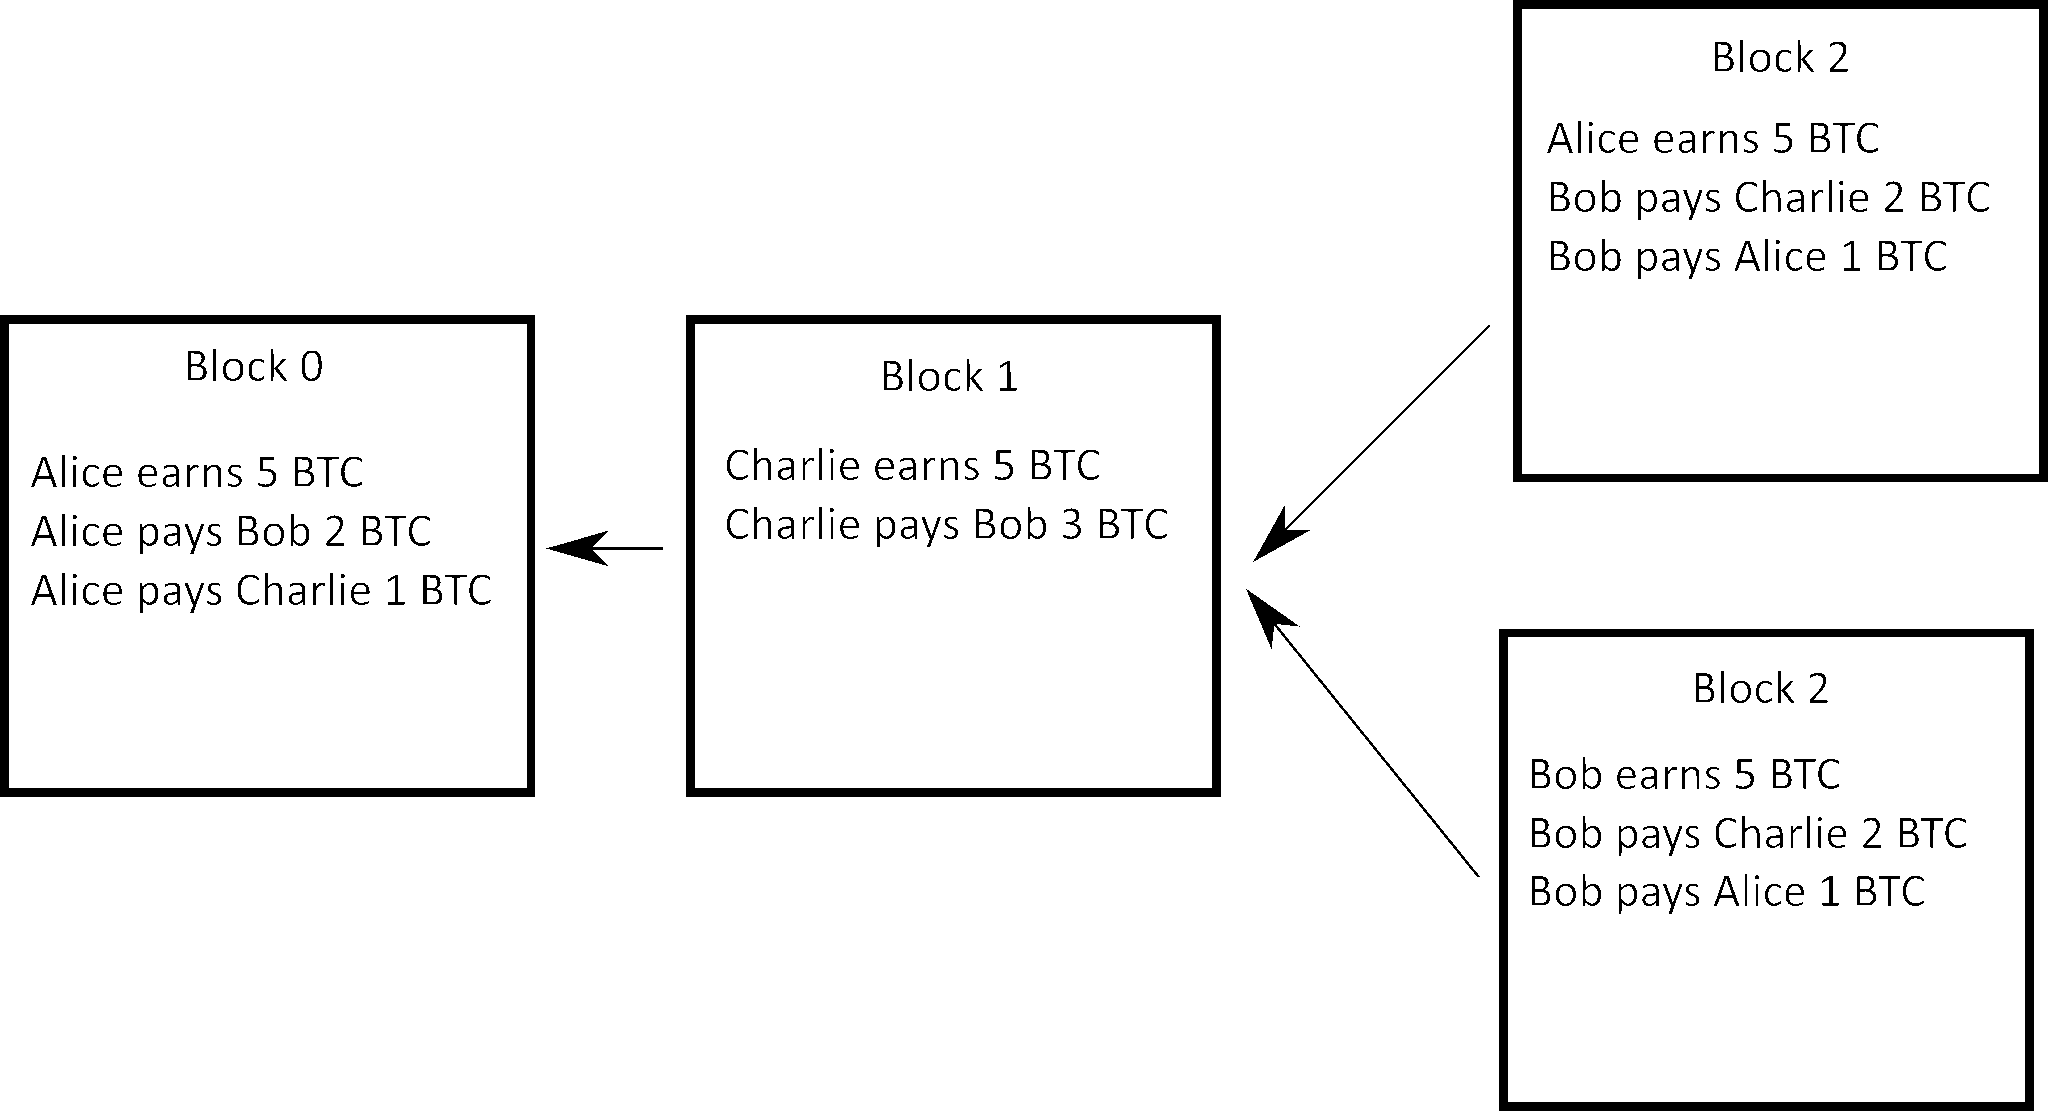
\includegraphics[width=\linewidth]{illustrationsSoutenance/forkEN.png}
	\end{figure}

\end{frame}


\begin{frame}

\frametitle{The fork problem}

\begin{figure}[H]
		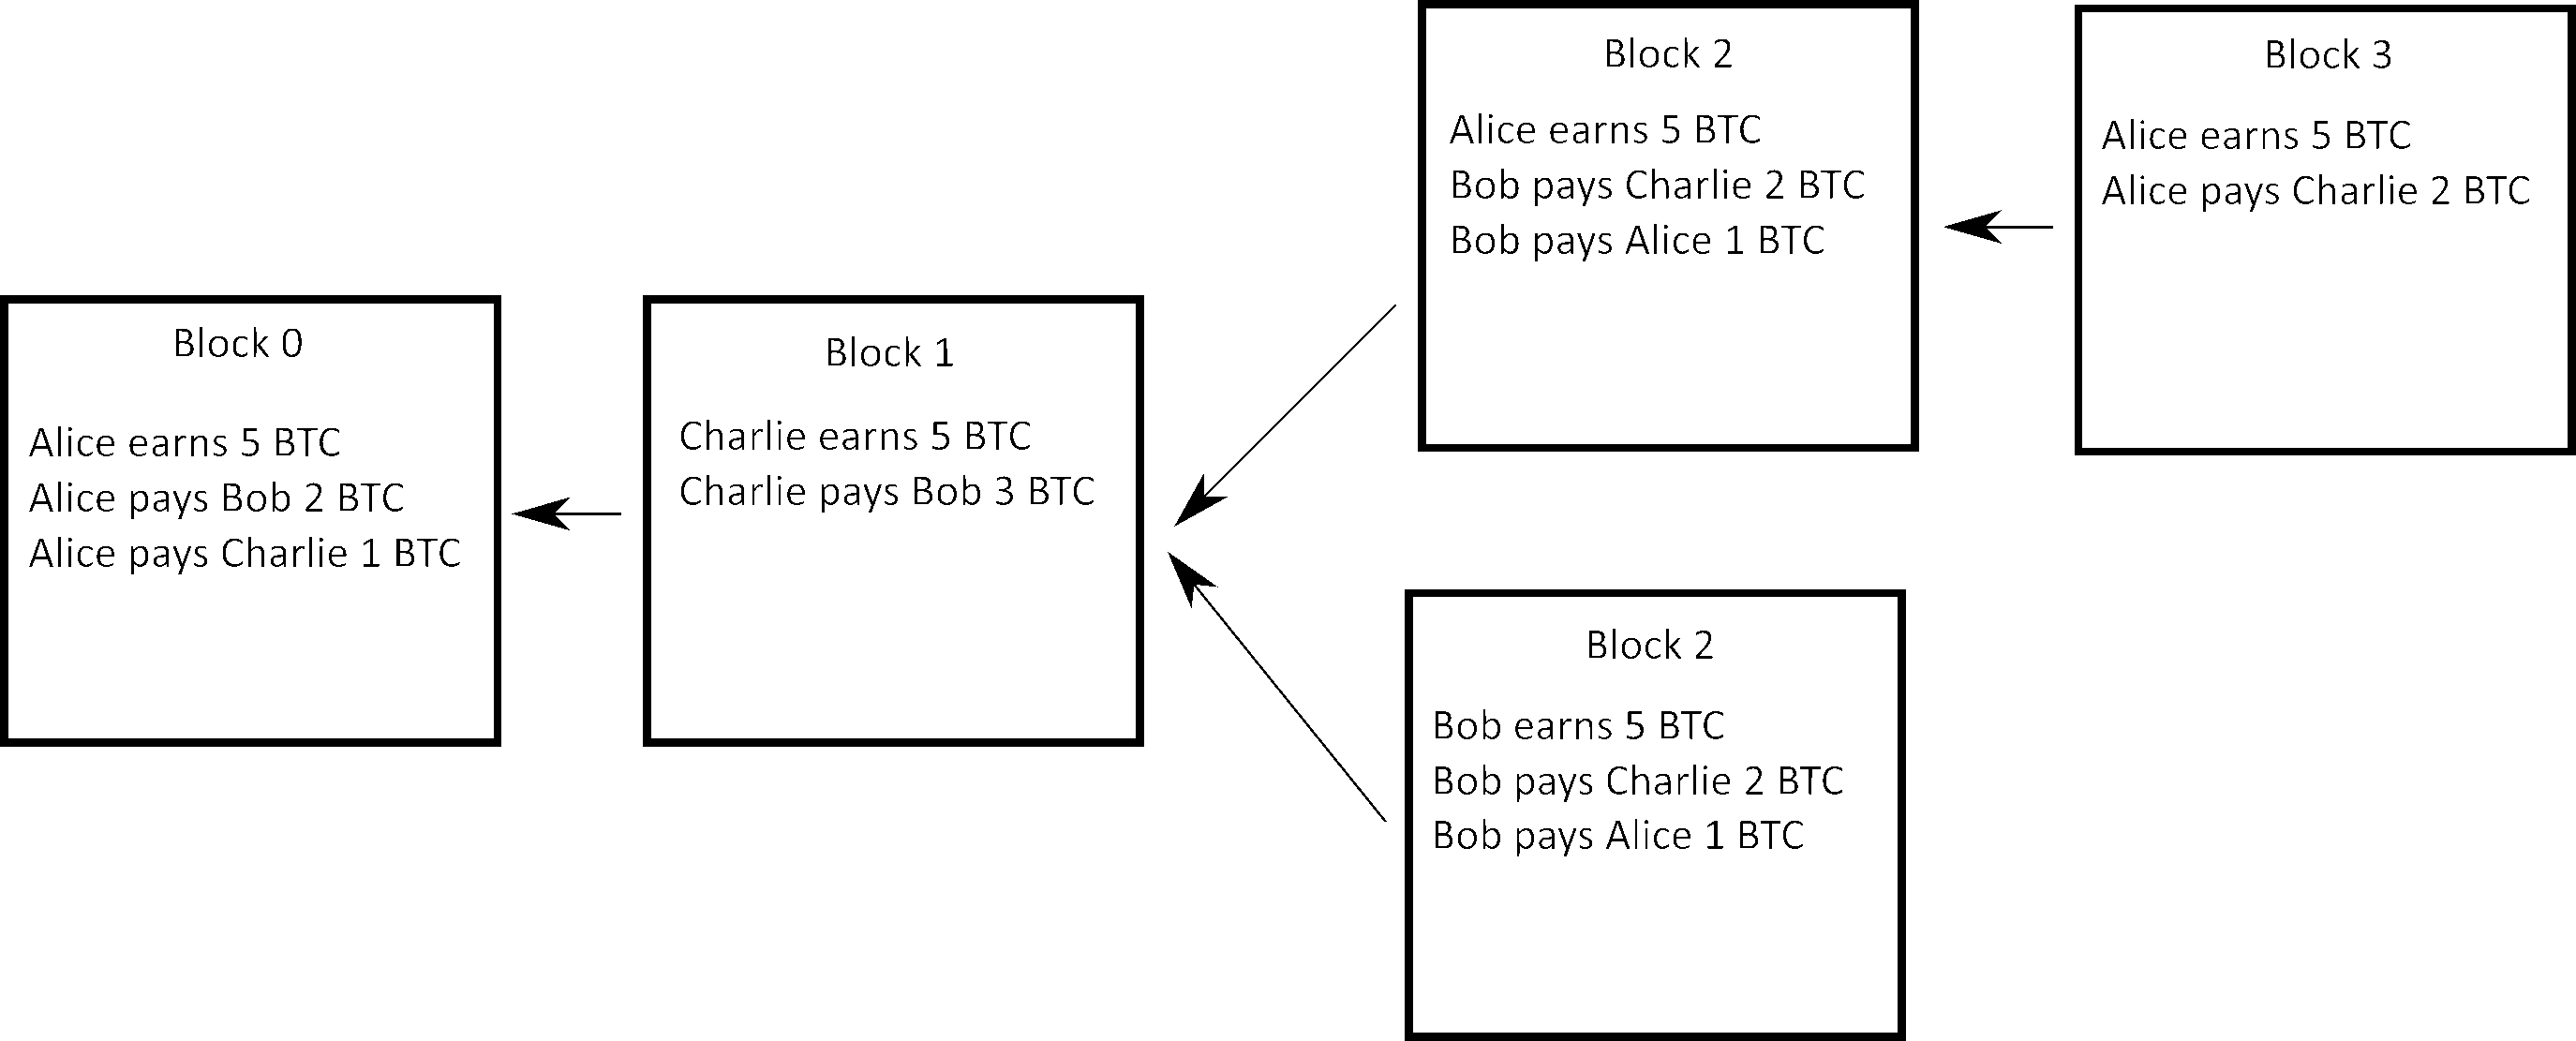
\includegraphics[width=\linewidth]{illustrationsSoutenance/forkContinueEN.png}
	\end{figure}

\end{frame}


\begin{frame}

\frametitle{The advantages of the theory}

\begin{figure}[H]
		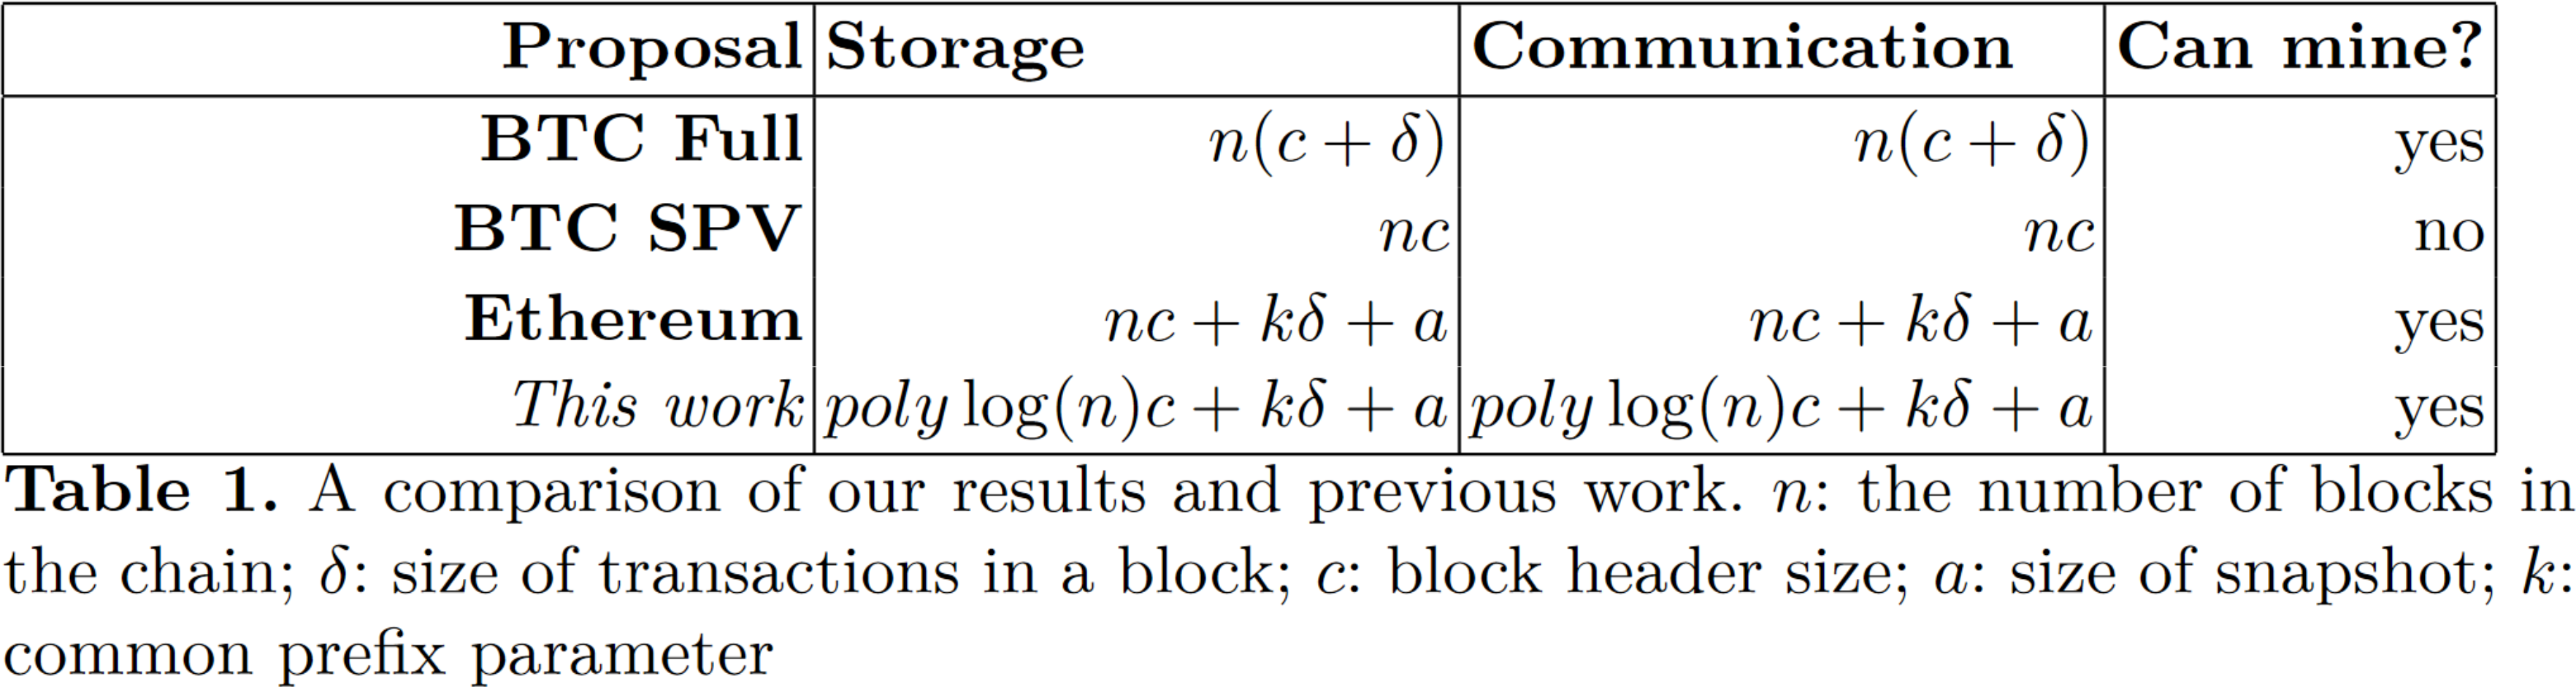
\includegraphics[width=\linewidth]{illustrations/tableauPage9.png}
		\caption{Excerpt from the table on page 9 of "Mining in Logarithmic Space" (BTC means Bitcoin)\\$n = 695 590$, $\delta$ between 0 and 2 Mb, $c = 97$, $a = 4.24$ Gb, $k = 6$}
	\end{figure}

\end{frame}

\begin{frame}

\frametitle{The interlink set problem}

\begin{figure}[H]
		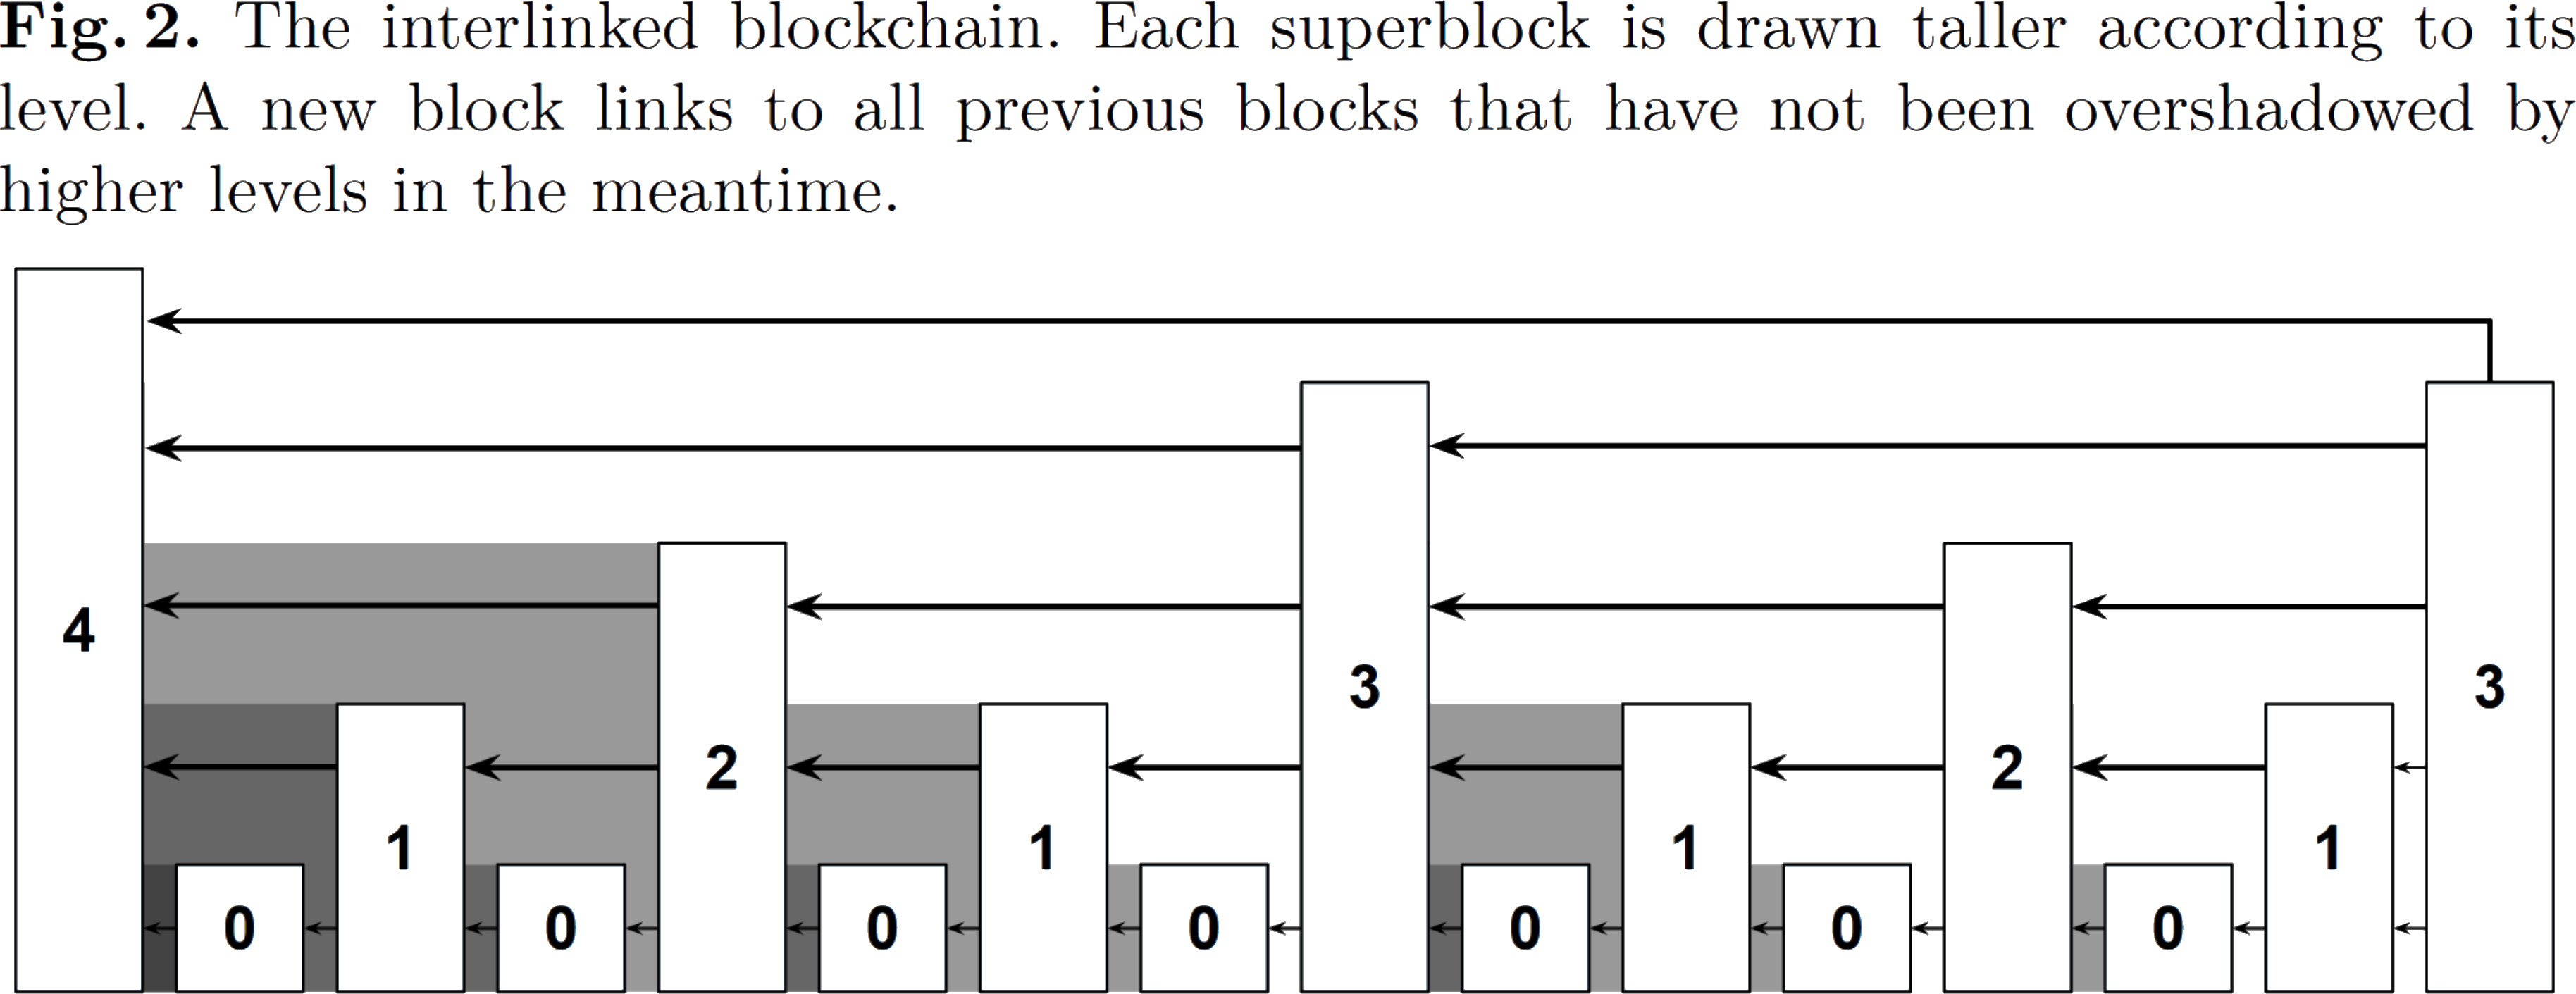
\includegraphics[width=\linewidth]{illustrations/interlinkSet.png}
		\caption{Set of "Mining in Logarithmic Space" pointers necessary for the proper execution of their approach}
	\end{figure}

\end{frame}

\begin{frame}

\frametitle{Some statistics}

\begin{figure}[H]
		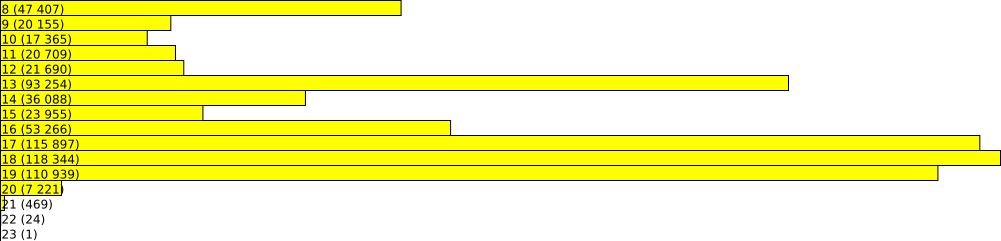
\includegraphics[width=\linewidth]{illustrations/hexaHashesStats.png}
		\caption{Distribution of Bitcoin block hashes by difficulty $m$ ($n$) where $m$ is the number of hexadecimal zeros at the beginning of the hash and $n$ the number of hashes beginning precisely with $m$ hexadecimal zeros}
	\end{figure}

\end{frame}

\begin{frame}

\frametitle{Some statistics}

%\vspace{-0.25cm}
		%\hspace{-3cm}
%\begin{figure}[H]
		%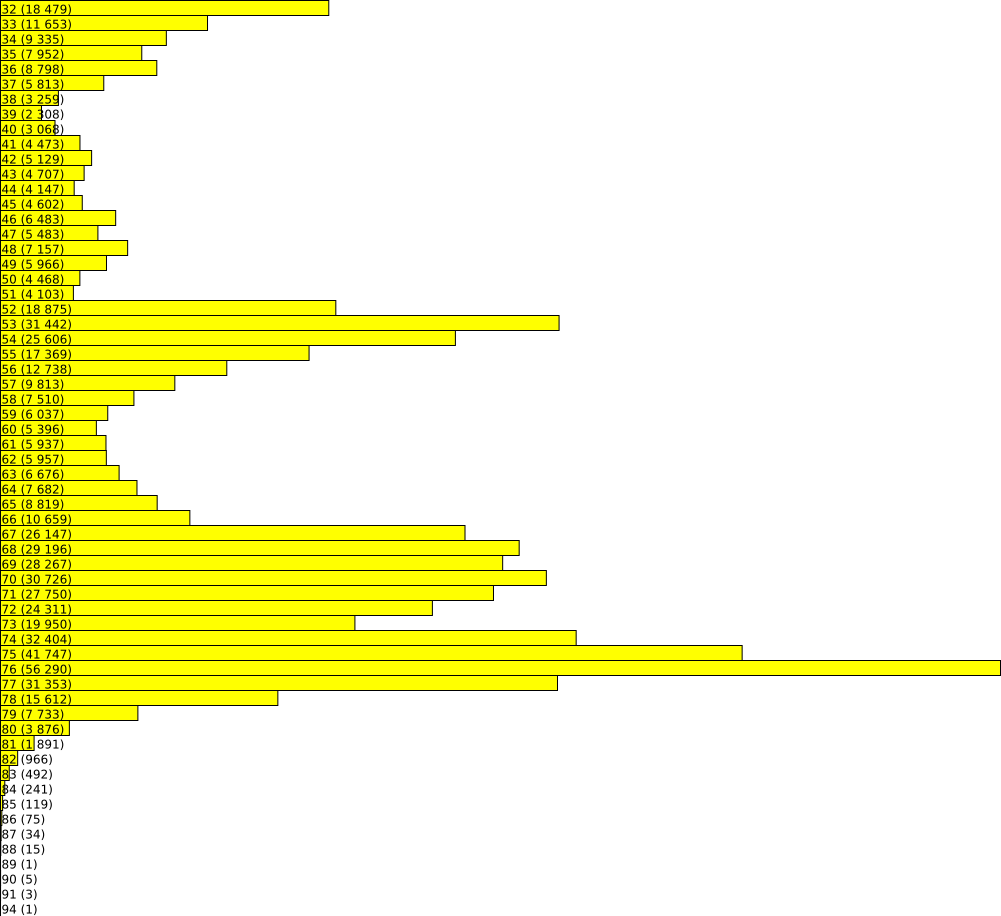
\includegraphics[width=0.85\linewidth]{illustrations/binHashesStats.png}
		%\hspace{5cm}
		%\vspace{-8cm}
		%\caption{Répartition des hachés des blocs de Bitcoin par difficulté $m$ ($n$) où $m$ est le nombre de zéros binaires au début du haché et $n$ le nombre de hachés débutant précisément par $m$ zéros binaires}
		%\begin{sidecaption}[fortoc]{title}[label]
%the body of the float
%\end{sidecaption}
	%\end{figure}
	
%	\begin{figure}
%\floatbox[{\capbeside\thisfloatsetup{capbesideposition={right,top},capbesidewidth=4cm}}]{figure}[\FBwidth]
%{\caption{A test figure with its caption side by side}\label{fig:test}}
%{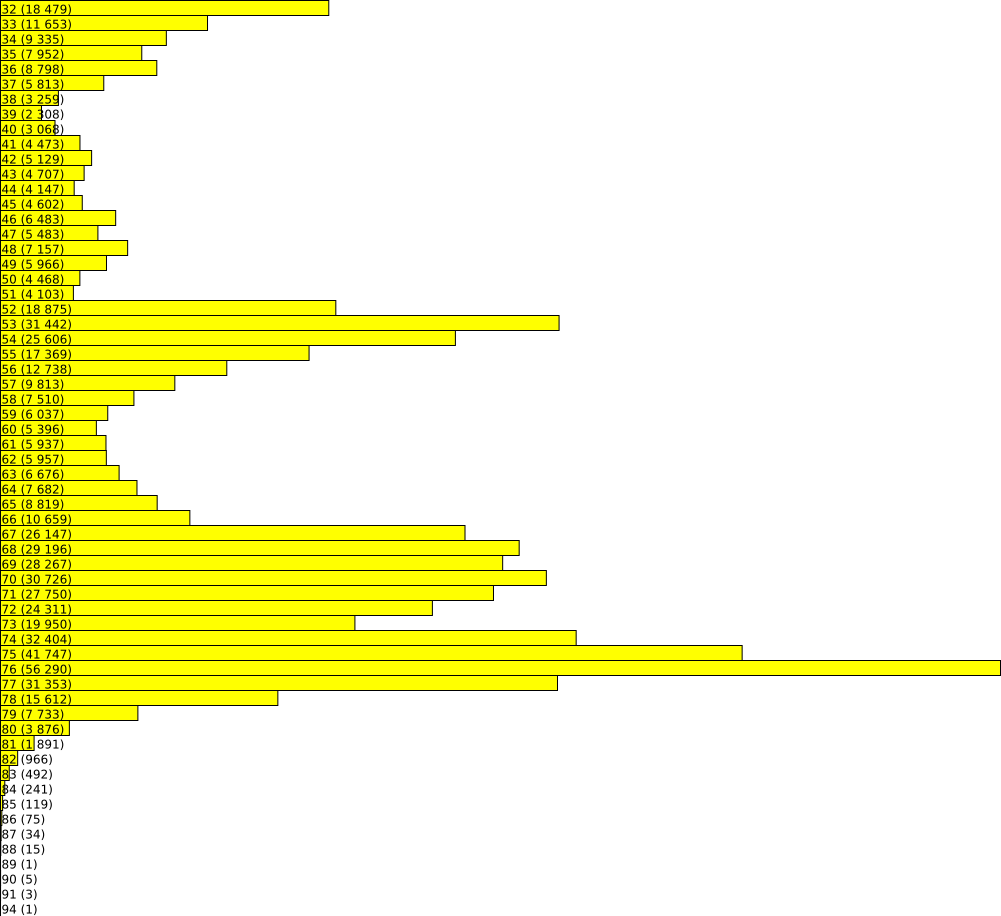
\includegraphics[width=5cm]{illustrations/binHashesStats.png}}
%\end{figure}

%\begin{SCfigure}
%    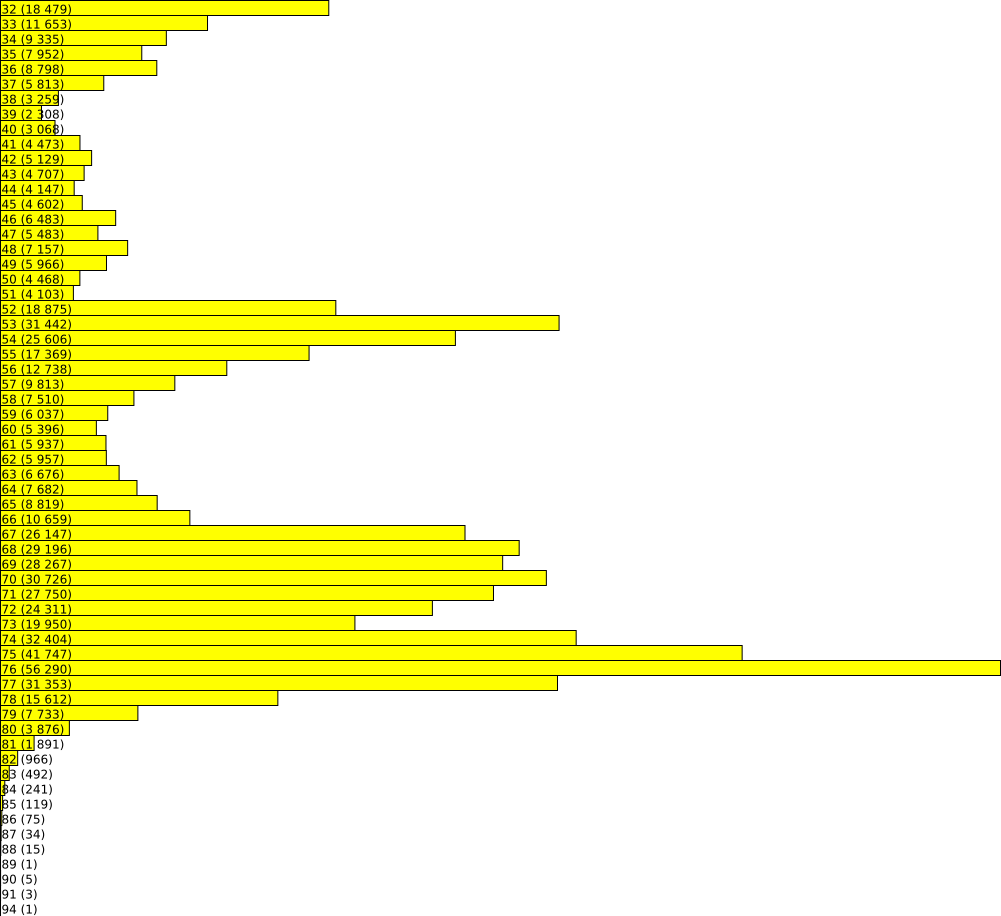
\includegraphics[width=5cm]{illustrations/binHashesStats.png}
%  \caption{Foo bar}
%\end{SCfigure}

\begin{figure}
      \begin{columns}
        \column{.8\linewidth}
        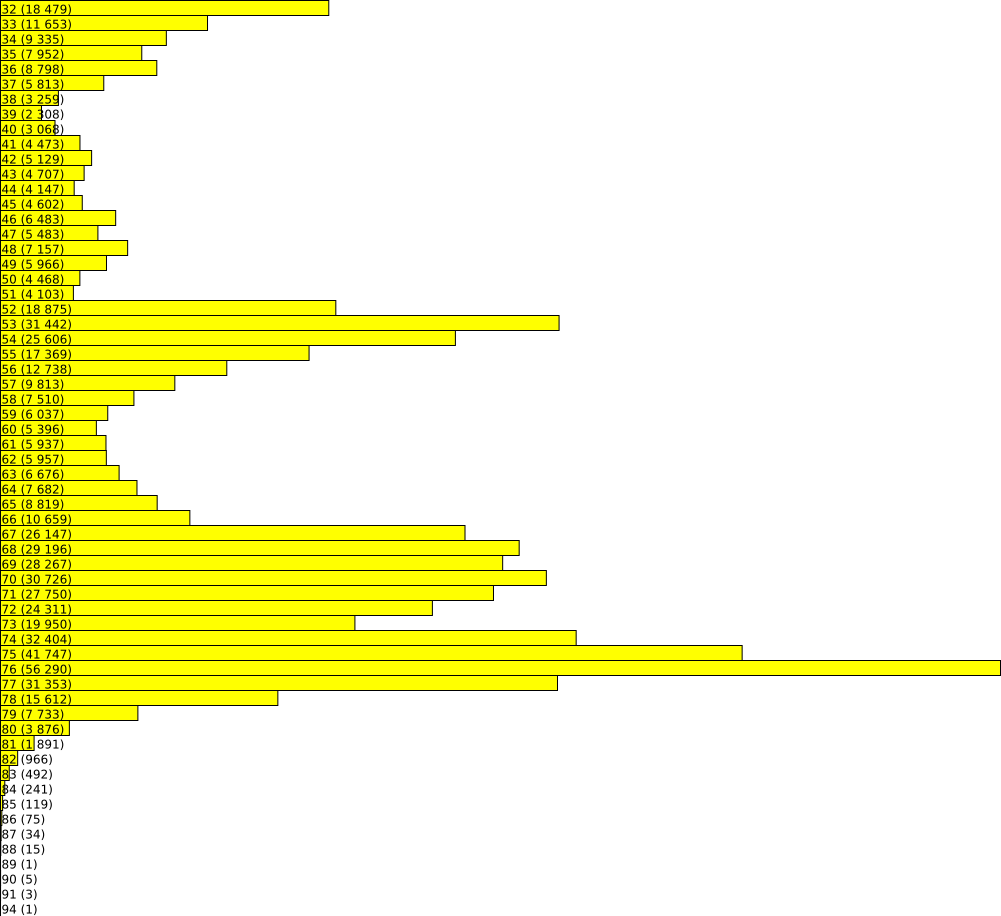
\includegraphics[width=\textwidth]{illustrations/binHashesStats.png}
        \column{.3\linewidth}
        \caption{Distribution of Bitcoin block hashes by difficulty $m$ ($n$) where $m$ is the number of binary zeros at the beginning of the hash and $n$ the number of hashes beginning precisely with $m$ binary zeros}
        \label{fig:example right}
      \end{columns}
    \end{figure}

%Test

\end{frame}

\begin{frame}

\frametitle{The compression algorithm}

%\vspace{-0.3cm}
\begin{figure}[H]
		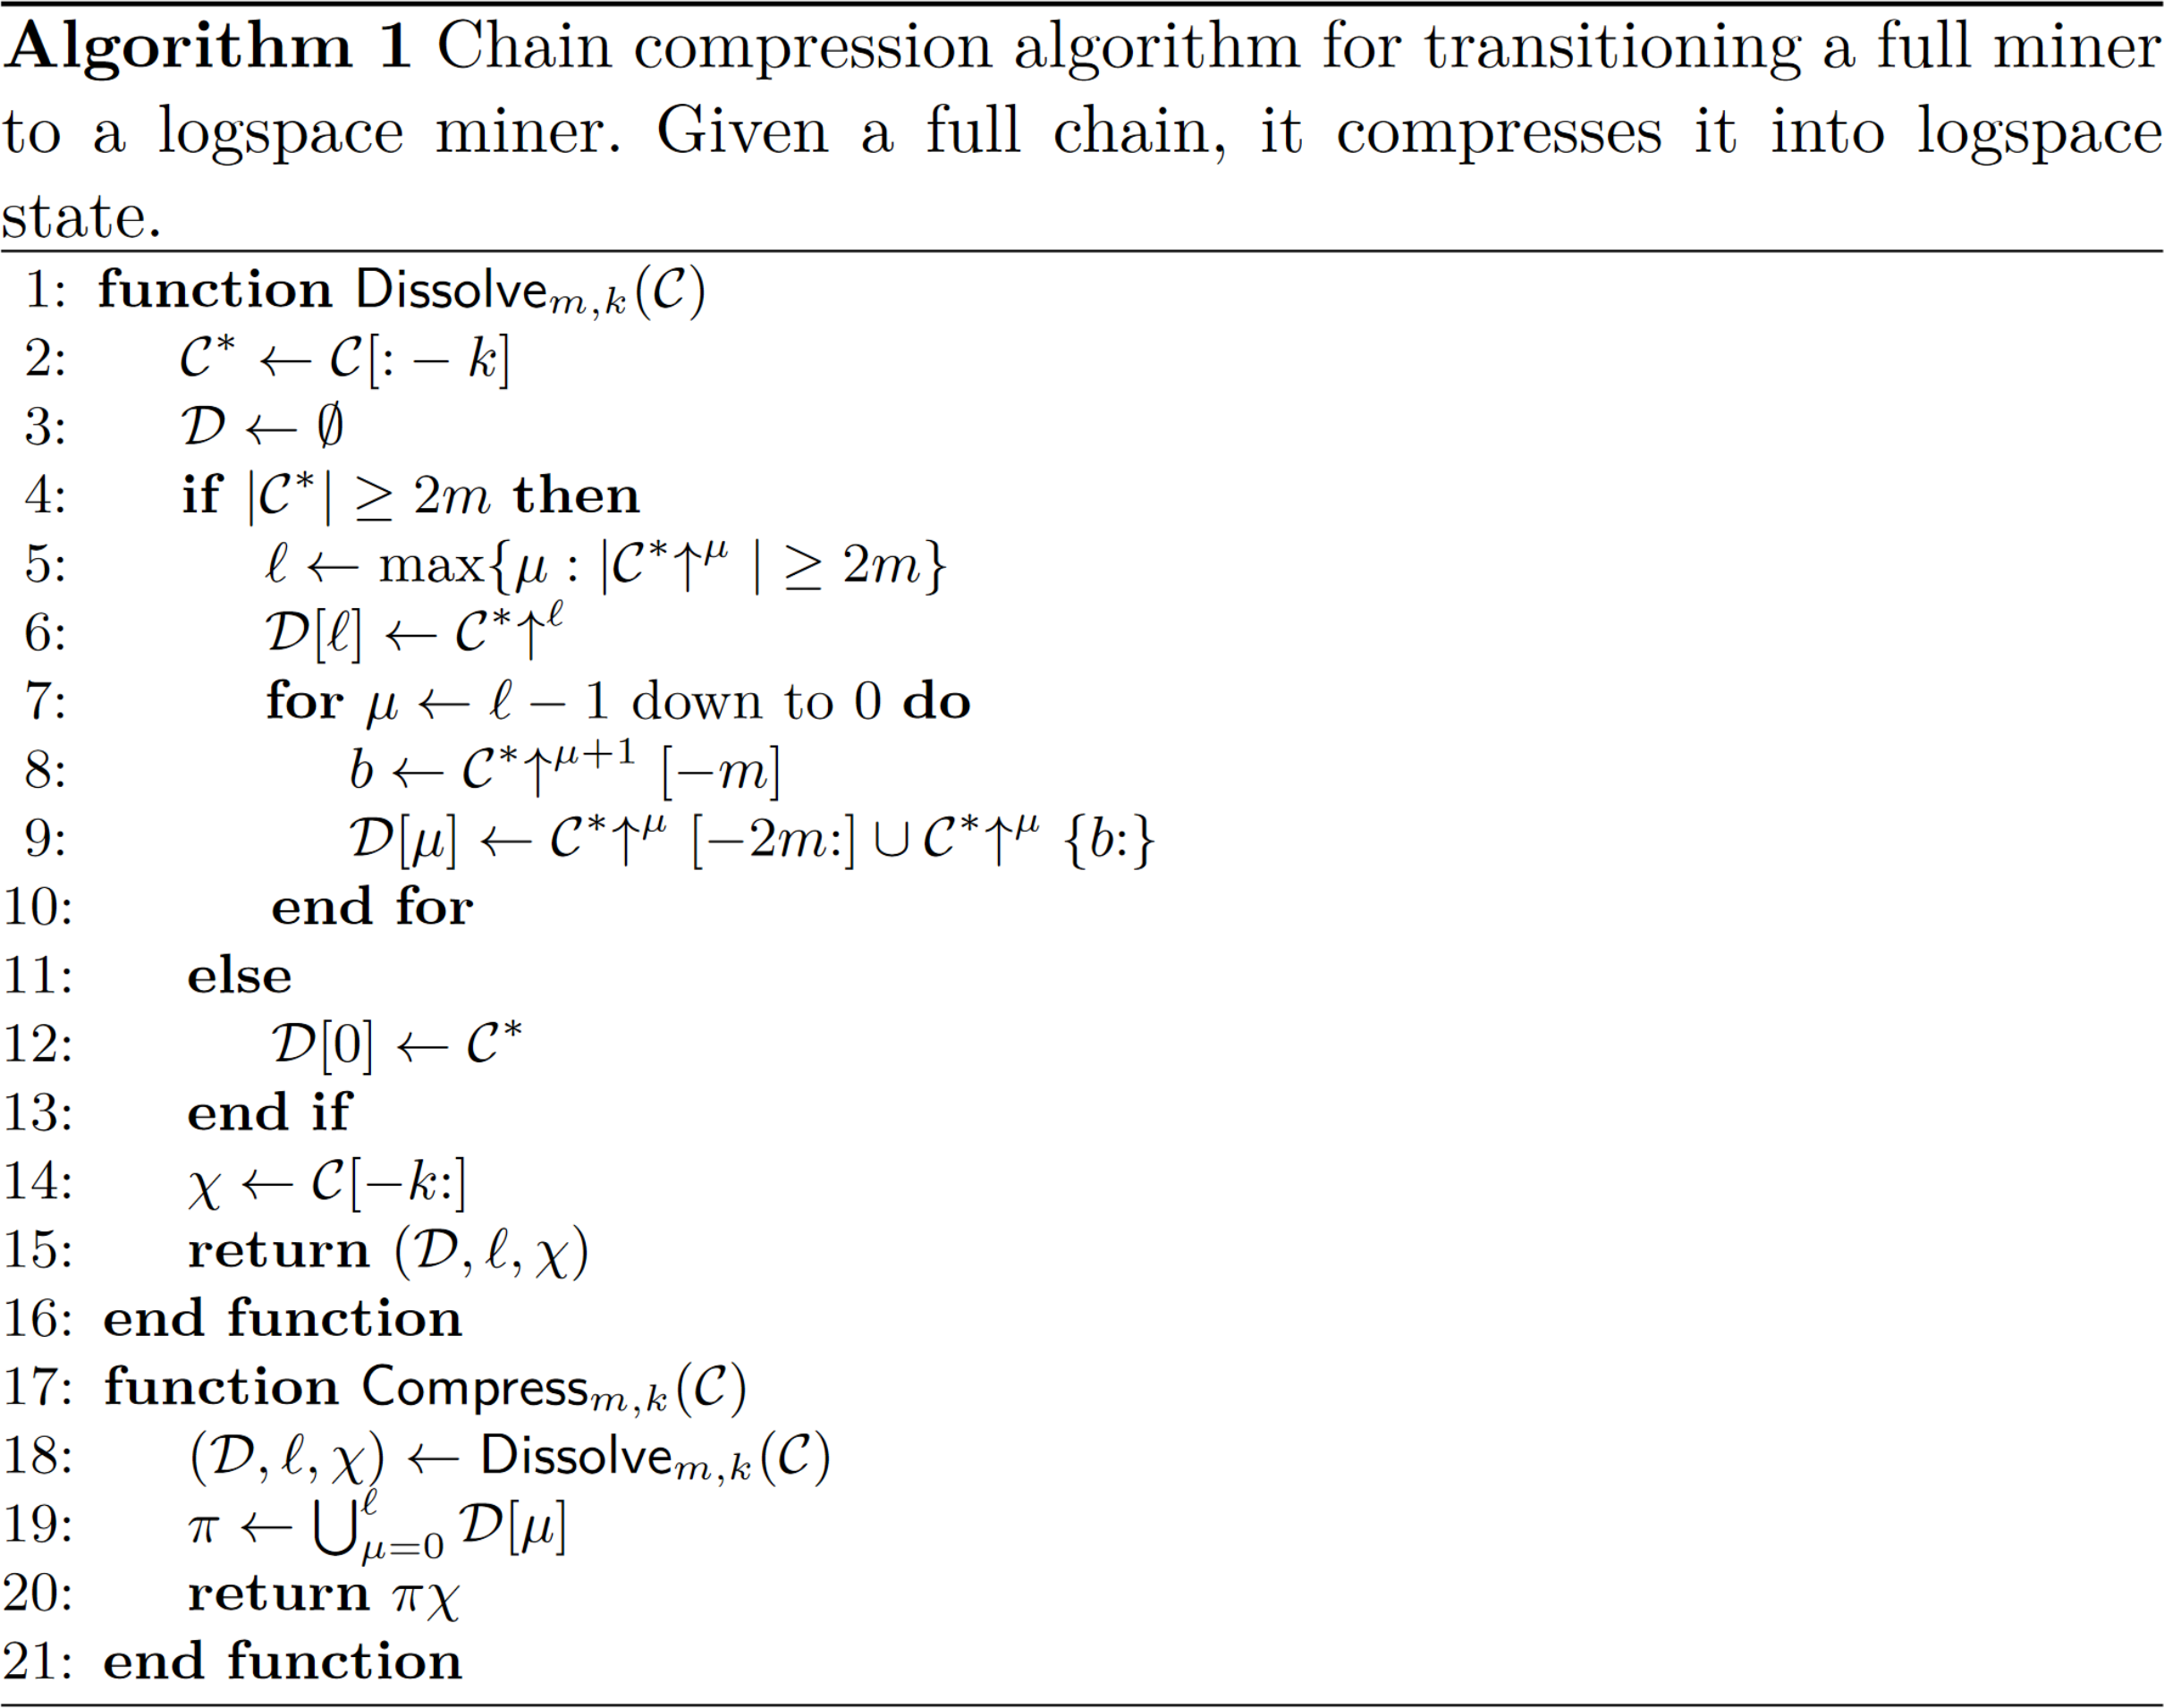
\includegraphics[width=0.7\linewidth]{illustrations/algo1.png}
		\caption{Algorithm 1 of "Mining in Logarithmic Space" allowing to compress a blockchain.\\$C$ is the blockchain\\$C^*\uparrow^\mu$ denotes blocks of exactly the same difficulty level $\mu$ of $C^*$\\$C^*\uparrow^\mu\{b:\}$ denotes blocks of $C^*\uparrow^\mu$ newer than the block $b$}
	\end{figure}

\end{frame}


\begin{frame}

\frametitle{The results}

\begin{figure}[H]
		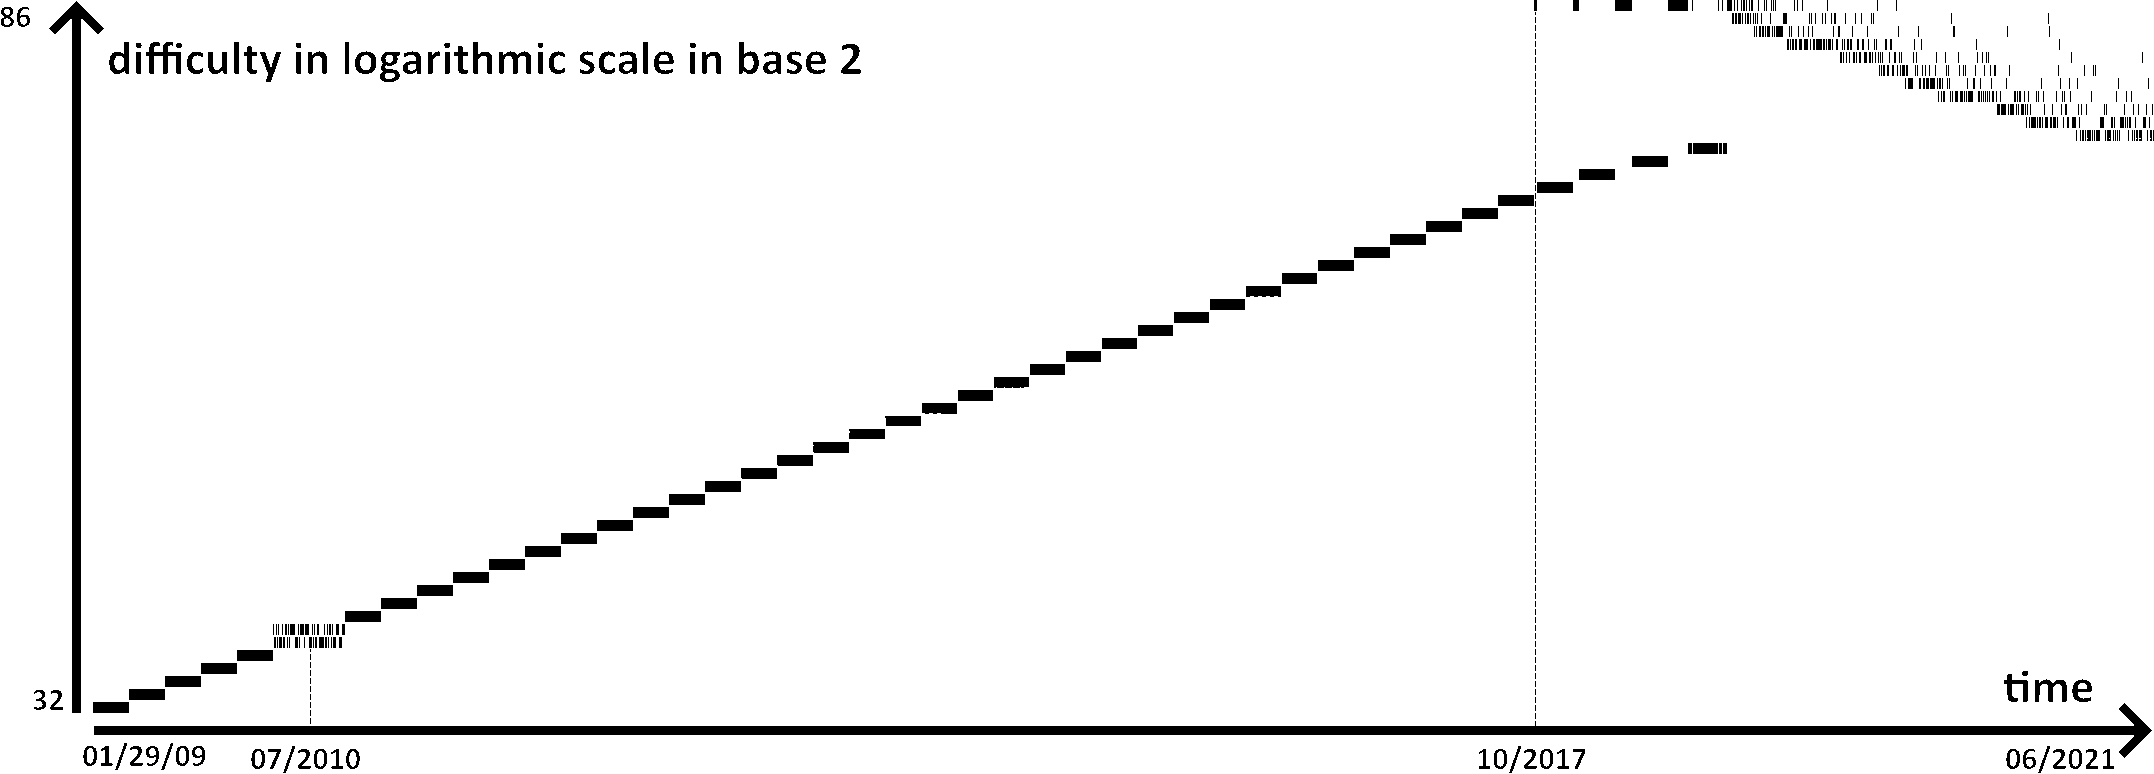
\includegraphics[width=\linewidth]{illustrations/piXEn.png}
		\caption{Distribution of the hashes of the blocks selected by the algorithm 1, where each block has a width of 1 pixel}%$\pi\chi$, où chaque bloc a une largeur de 1 pixel}
	\end{figure}

\end{frame}


\begin{frame}

\frametitle{Sources of illustrations}

	\begin{itemize}
		\item Page 2: Wikipedia: peer-to-peer
		\item Page 3: Blockchain.com
	\end{itemize}
\end{frame}

\end{document}